\chapter{Digital Marketplaces}
\label{ch:conceptual_framework_chapter}
To facilitate understanding the problem domain, it is necessary to briefly discuss the main elements in a digital marketplace and the key events that drive changes.
In this chapter, I draw inspirations from the research in temporal data mining \cite{adar2009temporal, aggarwal2015data} to better understand the phenomena of marketplaces.
I define the main concepts and terminologies in the context of digital marketplaces and how various elements interact in this ecosystem generating multiple events.
The goal is to highlight the broader impact and applications of the work presented in this dissertation.

\section{The Actions and the Changes}
Modern software platforms and technologies feature an online digital distribution platform called marketplace or store that allows users to discover and use digital artifacts made by third-party creators.
This platform created a thriving community of creators and users, which led to an exponential growth over a relatively short period of time.
In recent years, an increasing number of marketplaces enabled direct access of digital content or artifacts (e.g., software, multimedia files) to millions of users.
Marketplaces often take the form of an online store for a specific platform that allows creators to sell or distribute their products to users.
\begin{table}[h]
	\scalebox{1}{
		\begin{tabular}{ |p{4cm}|p{6cm}|p{5cm}| }
			\hline
			Marketplace & Platform & Size \\ \hline
			Pinshape.com & 3D-printable design files & 70,000+ makers and designers \\  \hline
			AWS marketplace &  Software and Cloud Services on Amazon Web Services &  2,200+ software systems and services \\ \hline
			Chrome Web Store &  Extensions and apps for the Chrome web browser &  18,000+ apps and thousands of extensions \\ \hline
			Windows Store &  Universal Apps on Microsoft Windows & 669,000+ apps \\ \hline
			iOS App Store &  Mobile Apps on iOS &  2,000,000+ apps \\ \hline
			Google Play &  Mobile apps on Android & 2,200,000+ apps  \\ \hline
			Amazon Appstore & Mobile apps on Android & 600,000+ apps \\
			\hline
		\end{tabular}
	}
	\caption{Several popular digital marketplaces for different platforms.}
	\label{tab:table_marketplaces}
\end{table}
Table~\ref{tab:table_marketplaces} shows a list of popular marketplaces for different platforms and the size of each marketplace \cite{statista_app_stores, pinshape, wikipedia_chrome_web_store}.
\begin{figure}[H]
	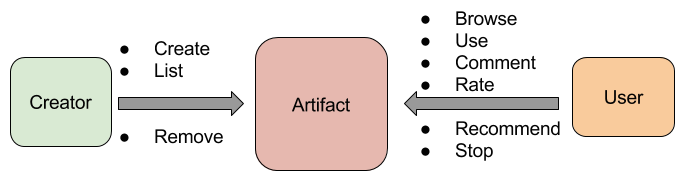
\includegraphics[scale=0.65]{figures/marketplaces/marketplace_single_artifact.png}
	\caption{The actions that a creator or a user may trigger to change the state of a single artifact. The creator triggers these actions once, while the user may trigger the actions multiple times.}
	\label{fig:figure_marketplace_actions_single}
	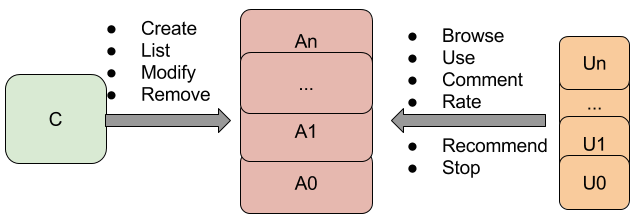
\includegraphics[scale=0.65]{figures/marketplaces/marketplace_multiple_artifacts.png}
	\caption{A chain of actions that a creator (C) or a user (U) may trigger to change the state of an artifact (A). The actions triggered by the creator results in a change to the state of the artifact or in a totally new artifact.}
	\label{fig:figure_marketplace_actions_multiple}
\end{figure}

The popularity of marketplaces as a means of distributing and sharing digital mediums in various platforms led to a growing community.
I define the key elements in this community as follows:
\begin{enumerate}
\item Creator (C): The person who is involved in the design, implementation, testing, and maintaining a digital artifact. A marketplace has a tuple of creators: $C=\{C_0, C_1,..., C_n\}$
\item User (U): The person who interacts with the digital artifact produced by the creator (C). In a marketplace, we will have a tuple of users: $U=\{U_0, U_1,..., U_n\}$
\item Artifact (A): Is a digital object made by a creator (C) to perform a task that benefits the user (U). In a marketplace, we will have a list of artifacts: $A=\{A_0, A_1,..., A_n\}$
\end{enumerate}
In addition, each of these elements is associated with custom actions that result in important events that describe or change the state of an artifact (depicted in figure~\ref{fig:figure_marketplace_actions_single}).
To model the actions that change the state of an artifact, consider a single artifact published at a marketplace by a single creator and used by multiple users.
This artifact can be a simple calculator app released in a mobile marketplace at some point of time, downloaded by multiple users, but never received an update.
This app represents the simplest form of the single-snapshot, and the time of observation is not considered important.
Installing this app now will always show the exact same view taken in its first and only version.
Thus, the view of the single-snapshot always matches the view of the time of its inception.
While marketplaces contain a considerable amount of artifacts that correspond to the ``single-snapshot'' model, a significant amount of artifacts are ever changing and thus do not fit into this model.

The nature of the marketplace is described as a dynamic sequence of events that results in complex changes to collection of artifacts.
For instance, consider an app that was published in a marketplace by a single creator, used by multiple users, reacted to multiple events, and evolved over time receiving multiple changes.
Figure~\ref{fig:figure_marketplace_actions_multiple} attempts to capture the factors and events that may contribute to the dynamic nature of the artifacts in the marketplace.
In this case, the creator's actions will often result in either a new artifact or a change to the state of the existing artifact, while the user's actions only result in a change to the state of the artifact (e.g., seen, used, recommended, etc.).
The common between all of these actions is the fact that they are associated with a series of time data that indicates when each action occurred.
A creator $C$ may observe the actions of a tuple of users: $\{U_0, U_1,..., U_n\}$ or react to external events which led to the changes or creation of new artifacts $\{A_0, A_1,..., A_n\}$ at different times $T=\{T_0, T_1,..., T_n\}$.
These time events are key to capturing and understanding the dynamic nature of marketplaces.
There are various challenges involved in capturing and analyzing the dynamic nature of the marketplace.
Perhaps the most difficult one is indicating which actions led to a change in the artifact.
This stems from the uncertainty in the events that led to a change in the state of the artifact, which is often caused by the lack of data that convincingly interpret the event.
The work and contributions presented in this dissertation aim to address the lack of data issue and motivate the creation of data-driven systems to answer complex analytical questions. 

\section{The Key Dimensions}
Although Chapter 3 provides a detailed review on previous related work, it is worth noting here that the vast majority of prior work in this area falls under the approach of studying the first model I referred to as the ``single-snapshot'' model.
While prior work in analyzing the content of marketplaces has yielded valuable results, it is often limited to the ``current moment'' of the finding.
The lack of investigating the dynamic and ephemeral nature of the artifacts in the marketplace leaves us unable to answer critical questions (e.g., how can we answer questions like: How did we get to this finding? Does this finding imply better outcome compare to the past? Can we predict if a different outcome is most likely to happen in the future?).
By viewing the digital marketplace as a dynamic, ever-evolving system, it opens up a new space for designing and conducting novel analyses to gain insights about this system, insights that are not possible with a single-snapshot view.
In this section, I describe the design space for such analysis methods for dynamic digital marketplaces.
To the best of my knowledge, this represents the first attempt to systematically map out this space.
The major dimensions of this space are: time resolution, inclusion criteria, and depth.

\subsection{Time Resolution}
Given the large amount of artifacts in marketplaces, a large number of observations may be made at different time points.
The first step in analyzing time series data is the selection of a specific frequency time span.
The precision of selecting a measurement of time is highly specific to the data analysis task.
This comes from the fact that different measurements of time frequency result in different observations.
In some cases, taking a longer measurement such as at each year or quarter will reveal patterns about slow changes.
This approach could be useful in observing slow changes and reporting on trends over a relatively longer period of time.
For example, when analyzing a list of artifacts in a marketplace, we can ask questions after taking a measurement at each year with respect to a specific design or development property.
This could enable us to ask questions like: what is the most popular design property in a given year? how popular is it in a different year? what was the increase in its popularity in another year?
In some cases, adjusting the measurement to a shorter period of time (e.g., monthly, weekly) may be considered a convenient way to sharpen the observations.
This short measurement is particularly useful in observing fast changes to digital artifacts in a marketplace.
For instance, we can ask questions like: what is the most changing design or development property over a given period? what are the top artifacts that made changes to this property?
To conclude, it is important to remember that the precise measurement of time may affect the outcome of the observations significantly.

\subsection{Inclusion Criteria}
This dimension is concerned with the selection of a subset of artifacts from a marketplace for analysis.
This problem has been studied extensively in statistics but it is worth to briefly discuss it here in the context of digital marketplaces.
One might begin by taking the approach of collecting the entire artifacts in the marketplace (i.e. conducting a census).
While it is obvious that this approach is expensive and requires lots of resources, there are reasons that his may not be the best approach.
The first reason is that access to the entire population is only possible to collect by the owners of the marketplace.
The second reason is that the population of artifacts change constantly in response to different actions and events, which means this approach will never result in a perfect measure of the population.
The more reasonable approach, however, is to collect a sample of the entire population of artifacts.
Sampling is easy to obtain and does not exhaust a lot of resources.
However,  sampling is often subject to error and bias.
For example, suppose that we attempt to estimate the existence of a certain design property in the artifacts in a marketplace.
If we collect a sample based on the top 10 artifacts from each category in a marketplace, then this sample would suffer from a selection bias because it is not a representative of the population.
We cannot make a valid conclusion about a collection of artifacts (i.e. statistical inference) when our sample suffers from bias.
Thus, it is important to conduct exploratory data analysis on the sample at hand to estimate the validity of the chosen sampling method.
There are a few sampling methods to consider and ensure that our sample is a representative of the population.
The commonly applied method is to randomly select artifacts from the marketplace such that each case is likely to be selected.
For example, one might start by taking a random sample of artifacts in a marketplace based on a randomly selected search terms.
If our sample does not suffer from sampling bias, we can generalize the observation to the entire population of artifacts.
The chosen inclusion criteria of our sample has to result in a representative sample of the population in order for the conclusion to be more reasonably valid.

\subsection{Depth}
This dimension is concerned with the internal and external parts an artifact is composed of.
A digital artifact consists of intrinsic and extrinsic parts that make up the artifact as a whole object.
These properties are essential to understanding the changes to the state of the artifact.
For example, consider a single digital artifact in a marketplace that has three part types:
a) Listing information on the marketplace that promotes it and describes its purpose.
b) Data that defines its visual appearance and how a user may interact with.
c) Data that describe its functional behavior.
An important characteristic of the changes in a digital marketplace is that a change at one of these levels may trigger another change at a different level.
For example, a developer may add changes to the functionality of the artifact.
This change may require changes to the data of the visual appearance to make it visible to users.
This change may also result in another change at the listing information level to promote the addition to users.
Therefore, we need consider all the parts that compose the artifact in order to understand the changes that occur to them over time and gain useful insights.

\section{Summary}
In this chapter, I formally defined the digital marketplace, its key elements, and how changes take place.
I discussed the limitations and problems that may arise when considering a single-snapshot approach.
I described how artifacts can be analyzed using a deep and longitudinal approaches.